\chapter{ANALISIS DAN PERANCANGAN}


\section{ANALISIS}

Sebagaimana telah dijelaskan pada \hyperref[ch:chapter_1]{Pendahuluan}, kegiatan perstatistikan di BPS dilakukan dengan mengacu kepada proses bisnis yang tertuang pada GSBPM. Dalam GSBPM, seperti pada Gambar ~\ref{fig:gsbpm2}, setiap kegiatan perstatistikan dilakukan dalam 8 fase: \textit{Specify needs}, \textit{Design}, \textit{Build}, \textit{Collect}, \textit{Process}, \textit{Analyze}, \textit{Disseminate}, dan \textit{Evaluate}. Tahap \textit{specify needs}, \textit{design}, dan \textit{build} merupakan tahapan-tahapan pada level perencanaan. Tahap \textit{collect} dan \textit{process} merupakan tahapan-tahapan pada level pelaksanaan. Sementara tahap \textit{analyze}, \textit{disseminate}, dan \textit{evaluate} merupakan tahapan-tahapan paska pelaksanaan.


Pada tahap \textit{collect}, data dikumpulkan dengan menggunakan media kuesioner. Sebagian besar kuesioner yang digunakan dalam pengumpulan data di BPS masih menggunakan media kuesioner kertas, meskipun beberapa \textit{survey} telah diujicobakan untuk menggunakan \textit{mobile device}. Sementara pada tahap \textit{process}, kuesioner yang telah terisi pada tahap \textit{collect} dilakukan \textit{editing}, \textit{coding}, dan imputasi. 


\subsection{Penyusunan Model Aplikasi} \label{ssec:analysis-application-model}

Berdasarkan hasil analisis dan studi literatur dari sejumlah pendekatan yang diusulkan, penggunaan \textit{mobile device} sebagai media pengumpulan data dapat diimplementasikan dalam dua pendekatan:

\begin{enumerate}
\item \hyperref[sssec:stand-alone]{Pendekatan \textit{stand alone}}
\item \hyperref[sssec:client-server]{Pendekatan \textit{client server}}
\end{enumerate}


\subsubsection{Pendekatan \textit{Stand Alone}} \label{sssec:stand-alone}

Pendekatan \textit{stand alone} merupakan model dimana semua \textit{resources} ditempatkan pada \textit{machine} tunggal \cite{li_collaborative_2005}. \textit{User interface}, \textit{services}, dan \textit{functions} semuanya berada pada \textit{machine} yang sama. Dalam keterkaitannya dengan pengumpulan data, dimana terdapat dua komponen utama yang harus terinstal pada \textit{device} yaitu \textit{user interface} dan data, maka keduanya terletak pada \textit{device} yang sama. Gambar ~\ref{fig:design-stand-alone} memberikan ilustrasi cara kerja pendekatan \textit{stand alone}, sementara Gambar ~\ref{fig:design-stand-alone-flowchart} menunjukkan alur kerja dari pendekatan \textit{stand alone}.


\begin{figure}[h]
    \centering
    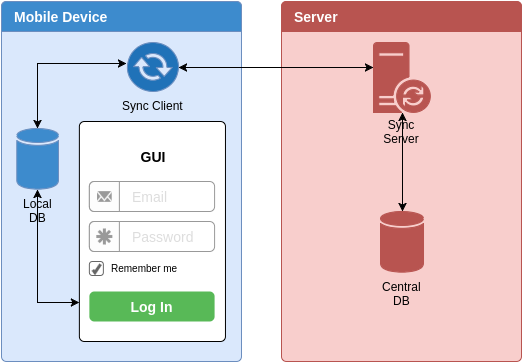
\includegraphics[width=.7\textwidth]{../../Resources/Images/design-stand-alone}
    \caption{Pendekatan \textit{Stand Alone}}
    \label{fig:design-stand-alone}
\end{figure}

\begin{figure}[h]
    \centering
    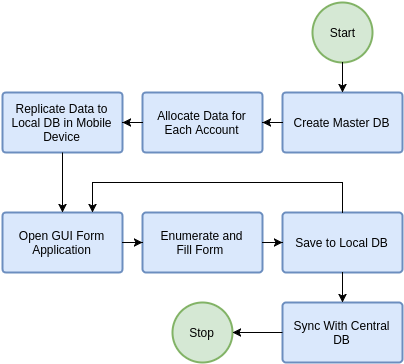
\includegraphics[width=.7\textwidth]{../../Resources/Images/design-stand-alone-flowchart}
    \caption{\textit{Flowchart} Pendekatan \textit{Stand Alone}}
    \label{fig:design-stand-alone-flowchart}
\end{figure}


Keuntungan dari pendekatan \textit{stand alone} adalah \textit{latency} yang terjadi pada saat \textit{client application} mengakses data menjadi lebih kecil dikarenakan letak data berada pada \textit{local machine}. Selain itu, pendekatan ini juga tidak memerlukan jaringan sebagai media komunikasi, sehingga sangat cocok digunakan pada \textit{disconnected environment}, dimana untuk kasus pengumpulan data lapangan kondisi ini akan sering dijumpai.


Sementara itu, pendekatan \textit{stand alone} memiliki sejumlah kelemahan, yaitu dalam hal data transfer dan pembaharuan aplikasi. Pendekatan stand alone tidak menggunakan media komunikasi untuk melakukan transfer data, sehingga diperlukan mekanisme transfer data manual untuk menggabungkan keseluruhan data. Selain itu, pembaharuan aplikasi juga harus dilakukan secara manual, sehingga perbaikan \textit{rule} validasi tidak akan dapat diakomodir secara otomatis.


Selain itu, pendekatan ini juga dapat digunakan pada \textit{disconnected environment}, dimana untuk kasus pengumpulan data lapangan kondisi ini akan sering dijumpai. Sementara itu, kelemahan pendekatan \textit{stand alone} ada pada letak eksekusi validasi yang terdapat pada sisi \textit{client}, sehingga perbaikan \textit{rule} validasi harus diikuti dengan pembaharuan aplikasi.


\subsubsection{Pendekatan \textit{Client Server}} \label{sssec:client-server}

Pendekatan \textit{client server} merupakan pendekatan yang telah banyak diadopsi \cite{schuster_client/server_1994} ~\cite{bertocco_client-server_1998} \cite{callaghan_clientserver_2007}. Secara abstrak, pendekatan \textit{client server} menghubungkan 2 (dua) bagian, \textit{client} dan \textit{server}. \textit{Server} menyediakan fungsi-fungsi, sementara program aplikasi (\textit{client}) melakukan eksekusi terhadap fungsi-fungsi tersebut \cite{schuster_client/server_1994}. Gambar \ref{fig:design-client-server-rpc} menunjukkan arsitektur \textit{client server} \textit{Remote Procedure Call} (RPC).

\begin{figure}[h]
    \centering
    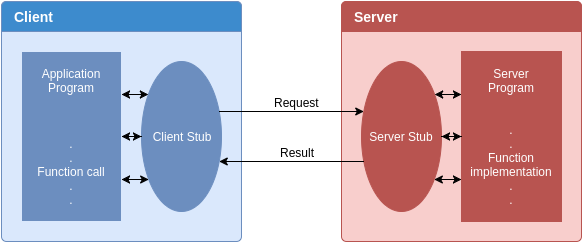
\includegraphics[width=.7\textwidth]{../../Resources/Images/design-client-server-rpc}
    \caption{\textit{Client Server} dengan RPC \cite{schuster_client/server_1994}}
    \label{fig:design-client-server-rpc}
\end{figure}


Implementasi pendekatan \textit{client server} dalam konteks pengumpulan data menggunakan \textit{mobile device} sebagai \textit{client}. Pada pendekatan ini data diletakkan berdekatan dengan \textit{server}, sehingga \textit{device} perlu mengaksesnya secara \textit{remote}. Gambar \ref{fig:design-client-server} memberikan ilustrasi penggunaan pendekatan \textit{client server} dalam pengumpulan data lapangan. Sementara Gambar \ref{fig:design-client-server-flowchart} menunjukkan alur kerja dari pendekatan \textit{client server}.


Kelemahan yang dimiliki pendekatan \textit{client server} adalah, untuk dapat digunakan, \textit{client application} harus selalu terkoneksi dengan \textit{central server} dimana data berada, sehingga pendekatan ini tidak dapat digunakan pada \textit{disconnected environment}. Selain itu, setiap kali \textit{client application} melakukan komunikasi dengan \textit{central server}, maka sejumlah data akan ditransmisikan, sehingga diperlukan kapasitas dan kapabilitas jaringan yang cukup baik kuota maupun \textit{transfer rate}. 

\begin{figure}[h]
    \centering
    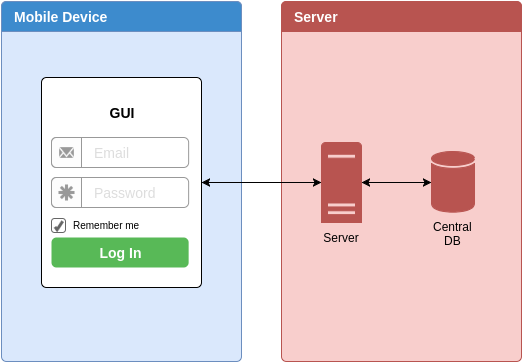
\includegraphics[width=.7\textwidth]{../../Resources/Images/design-client-server}
    \caption{Pendekatan \textit{Client Server}}
    \label{fig:design-client-server}
\end{figure}

\begin{figure}[h]
    \centering
    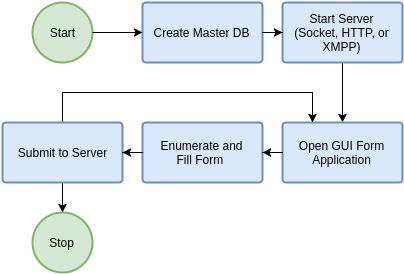
\includegraphics[width=.7\textwidth]{../../Resources/Images/design-client-server-flowchart}
    \caption{\textit{Flowchart} Pendekatan \textit{Client Server}}
    \label{fig:design-client-server-flowchart}
\end{figure}


Sebagaimana telah diketahui, pengumpulan data merupakan suatu kegiatan yang memerlukan mobilitas. Petugas perlu  berkeliling untuk mengunjungi responden secara \textit{door-to-door}. Pendekatan \textit{client-server} memerlukan ketergantungan yang tinggi terhadap sinyal komunikasi, sementara kondisi lapangan tidak selalu mendukung tersedianya sinyal komunikasi. Di sisi lain, pendekatan \textit{stand alone} memiliki kelemahan dalam proses transfer data yang harus dilakukan secara manual. 


Berdasarkan analisis terhadap kebutuhan dalam pengumpulan data dengan menggunakan \textit{mobile device}, maka desain yang dirancang harus mempertimbangkan kriteria berikut:

\begin{enumerate}
\item Mendukung \textit{disconnected environment} \\
Pengumpulan data memerlukan penyisiran lapangan dengan kondisi geografis yang bervariasi. Kondisi sinyal telekomunikasi pada masing-masing wilayah pendataan juga bervariasi, dari yang bagus sampai yang tidak terdapat sinyal komunikasi. Desain yang dirancang harus dapat mengakomodir pengumpulan data pada wilayah yang tidak terdapat sinyal komunikasi.

\item Mendukung pembaharuan secara otomatis \\
Kuesioner elektronik yang terinstal pada \textit{device} merupakan representasi dari variabel sensus/survei yang akan dikumpulkan. Dalam pengisiannya, ada aturan \textit{rule} validasi yang harus diikuti, sehingga pembaharuan \textit{rule} validasi diperlukan ketika ada perbaikan konsep dan definisi.
\end{enumerate}


\section{PERANCANGAN}

\subsection{Perancangan Model Aplikasi}

Secara garis besar, terdapat 2 (dua) jenis \textit{object} yang menjadi poin utama dari solusi yang akan dirancang, yaitu: data dan \textit{rule} validasi. Agar mendukung \textit{disconnected environment}, maka diperlukan adanya mekanisme replikasi data. Sementara agar data senantiasa \textit{up-to-date}, diperlukan juga adanya mekanisme sinkronisasi. Secara umum, solusi yang akan dirancang akan memiliki arsitektur seperti pada Gambar \ref{fig:architecture-solution}.

\begin{figure}[h]
    \centering
    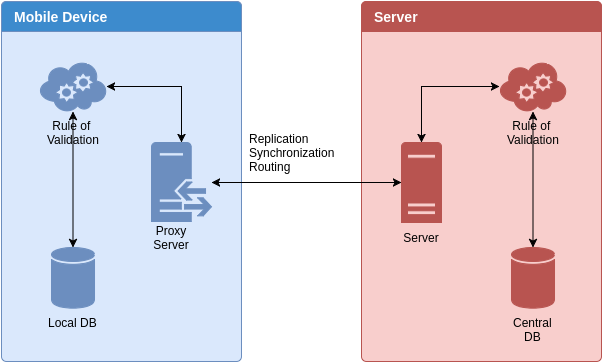
\includegraphics[width=.87\textwidth]{../../Resources/Images/architecture-solution}
    \caption{Arsitektur Solusi}
    \label{fig:architecture-solution}
\end{figure}


\subsection{Replikasi}

Replikasi merupakan suatu cara untuk memastikan agar baik \textit{device} maupun \textit{server} mengeksekusi objek yang sama. Replikasi dilakukan satu arah, yaitu dari \textit{server} ke \textit{device}. Terdapat 2 (dua) jenis mekanisme replikasi yang dirancang, yaitu: replikasi rule dan replikasi data.


\subsubsection{Replikasi \textit{Rule} Validasi}

\textit{Rule} validasi ada implementasi dari \textit{logic workflow}, seperti yang tertuang pada GSBPM fase \textit{Build} subproses \textit{Configure Workflows}. Replikasi \textit{rule} validasi bertujuan agar validasi isian kuesioner dapat dijalankan secara lokal. Implementasi \textit{rule} validasi dikemas dalam format \textit{OSGI Bundle}. Gambar ~\ref{fig:architecture-rule-replication} menunjukkan skema replikasi \textit{rule} validasi.

\begin{figure}[h]
    \centering
    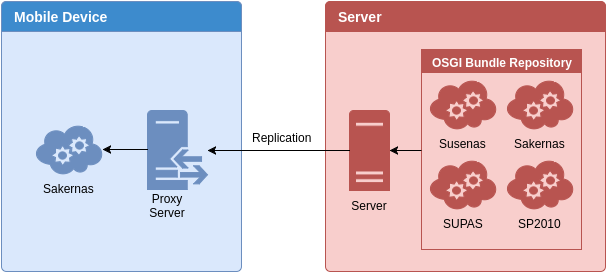
\includegraphics[width=.93\textwidth]{../../Resources/Images/architecture-rule-replication}
    \caption{Skema Replikasi \textit{Rule} Validasi}
    \label{fig:architecture-rule-replication}
\end{figure}


\subsubsection{Replikasi Data}

\textit{Rule} validasi selain memuat \textit{logic workflow} juga memuat \textit{object} yang merupakan representasi dari tabel di \textit{database} yang disebut dengan \textit{Object Relational Mapping (ORM)}. Tidak semua data diperlukan, sehingga replikasi harus dilakukan secara selektif. ORM inilah yang akan menentukan tabel dan data apa saja yang akan di replikasi. Gambar ~\ref{fig:architecture-data-replication} menunjukkan skema replikasi data.

\begin{figure}[h]
    \centering
    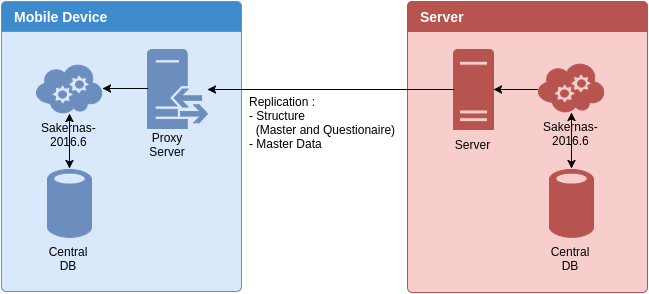
\includegraphics[width=.93\textwidth]{../../Resources/Images/architecture-data-replication}
    \caption{Skema Replikasi Data}
    \label{fig:architecture-data-replication}
\end{figure}


\subsection{Sinkronisasi}

Seperti halnya replikasi, sinkronisasi juga bertujuan untuk memastikan \textit{device} dan \textit{server} mengeksekusi objek yang sama. Akan tetapi, sinkronisasi berjalan sepanjang waktu, baik melalui \textit{scheduler} maupun \textit{trigger}. Selain itu, sinkronisasi dilakukan dua arah, dari \textit{server} ke \textit{device} maupun dari \textit{device} ke \textit{server}, tergantung \textit{object} yang sedang dieksekusi. Terdapat 2 (dua) jenis mekanisme sinkronisasi yang dirancang, yaitu: sinkronisasi rule dan sinkronisasi data.


\subsubsection{Sinkronisasi \textit{Rule} Validasi}

Sinkronisasi \textit{rule} validasi menggunakan implementasi yang sama dengan replikasi \textit{rule} validasi. Perbedaanya, sinkronisasi \textit{rule} validasi menggunakan \textit{trigger} yang berupa versi. Setiap kali \textit{client application} menemukan pembaharuan versi \textit{rule} validasi pada server, maka \textit{client application} secara otomatis akan memperbarui \textit{rule} validasinya. Gambar ~\ref{fig:architecture-rule-synchronization} menunjukkan skema sinkronisasi \textit{rule} validasi.

\begin{figure}[h]
    \centering
    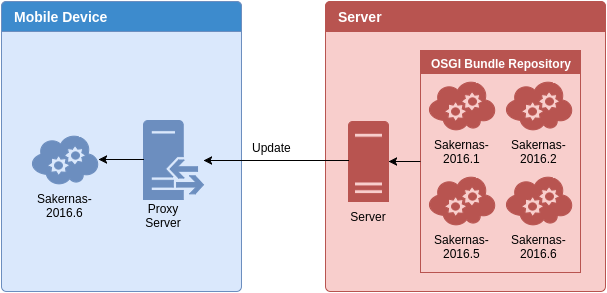
\includegraphics[width=.93\textwidth]{../../Resources/Images/architecture-rule-synchronization}
    \caption{Skema Sinkronisasi \textit{Rule} Validasi}
    \label{fig:architecture-rule-synchronization}
\end{figure}


\subsubsection{Sinkronisasi Data}

Sebagaimana yang telah dijabarkan dalam analisis, terdapat 2 (dua) jenis data yang dikelola, yaitu: data \textit{master} dan data lapangan. Arah sinkronisasi data menyesuaikan jenis data-nya. Data master pada \textit{server} diasumsikan lebih \textit{up-to-date}, sehingga sinkronisasi dilakukan dari arah \textit{server} ke \textit{device}. Sebaliknya, data lapangan pada \textit{device} diasumsikan lebih \textit{up-to-date}, sehingga sinkronisasi dilakukan dari arah \textit{device} ke \textit{server}. Gambar ~\ref{fig:architecture-data-synchronization} menunjukkan skema sinkronisasi data.

\begin{figure}[h]
    \centering
    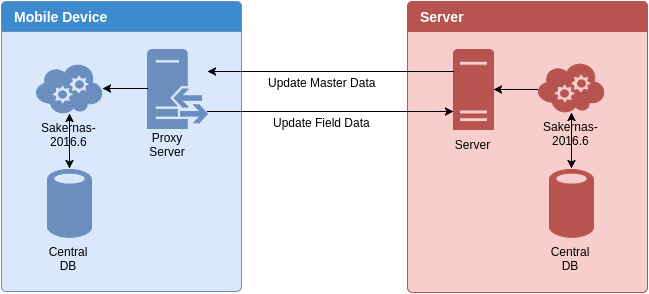
\includegraphics[width=.93\textwidth]{../../Resources/Images/architecture-data-synchronization}
    \caption{Skema Sinkronisasi Data}
    \label{fig:architecture-data-synchronization}
\end{figure}


\subsection{Routing}

Proses \textit{routing} menggunakan sebuah \textit{proxy server}. \textit{Proxy server} berperan sebagai \textit{Application-Level Gateway (ALG)} yang menyediakan fungsi \textit{security}, \textit{filtering}, dan \textit{packet forwarding}. 


\subsection{Pengelolaan Data}

Sesuai dengan model aplikasi yang akan dirancang, yaitu pendekatan \textit{client server} dengan \textit{proxy}, terdapat 2 (dua) jenis penyimpanan data, yaitu pada sisi \textit{client} dan sisi \textit{server}. Agar kedua sisi penyimpanan data tersebut merepresentasikan data yang sama, maka terdapat mekanisme pengelolaan data yang harus diikuti.

Dalam kegiatan pengumpulan data lapangan, terdapat 2 (dua) jenis data yang digunakan:

\begin{enumerate}
\item Data \textit{master} \\
Data \textit{master} merupakan data yang digunakan sebagai referensi oleh variabel pendataan. Data \textit{master} bersifat \textit{non-volatile}, yang artinya tidak mudah berubah. Perubahan data master hanya dapat dilakukan pada \textit{phase} design pada GSBPM. Contoh data \textit{master} antara lain: data master wilayah, data master status perkawinan, data master status dalam rumah tangga, dll.

\item Data lapangan \\
Data lapangan merupakan data yang isinya merupakan representasi hasil pendataan. Data ini bersifat transaksional, artinya data dapat dengan mudah ditambah, dihapus, maupun di\textit{update}. Contoh data lapangan antara lain: data sakernas semester I 2016, data susenas semester I 2016, data usaha rumah tangga pertanian ST2016, dll.
\end{enumerate}


Secara umum, variabel yang sejenis yang digunakan pada beberapa sensus maupun survei mempunyai konsep dan definisi yang sama, misalnya: Variabel jenis kelamin pada Sakernas \footnote{\url{https://sirusa.bps.go.id/index.php?r=variabel/view&id=11482}}, Susenas \footnote{\url{https://sirusa.bps.go.id/index.php?r=variabel/view&id=12526}}, SUPAS \footnote{\url{https://sirusa.bps.go.id/index.php?r=variabel/view&id=11341}}, dll, mempunyai konsep dan definisi, serta atribut yang sama, yaitu: 1 - laki-laki, 2 - perempuan. Begitu pula variabel-variabel yang lain, digunakan secara bersamaan oleh beberapa sensus dan survei.


Dari hasil analisis berdasarkan jenis-jenis data dan karakteristik variabel yang digunakan, maka dapat dirangkum dalam beberapa poin berikut:

\begin{enumerate}
\item \textit{Server} memuat seluruh data \textit{master} yang digunakan pada seluruh kegiatan sensus dan survei.
\item \textit{Client} memuat hanya data \textit{master} yang digunakan oleh kegiatan tertentu sana.
\item Data \textit{master} bersifat \textit{non-volatile}, sehingga diasumsikan data master pada \textit{server} lebih \textit{up-to date} dibandingkan data master pada \textit{client}. Oleh karena itu, replikasi data \textit{master} dilakukan dari \textit{server} ke \textit{client}.
\item Data lapangan bersifat transaksional, artinya data lapangan pada \textit{client} diasumsikan kondisinya lebih \textit{up-to date} dibandingkan data lapangan pada \textit{server}. Oleh karena itu, replikasi data lapangan dilakukan dari \textit{client} ke \textit{server}.
\end{enumerate}
